\chapter{Óvintézkedések}\label{ch:precautions}

Ez a fejezet összegyűjti azokat a kötelező biztonsági előírásokat, amelyek minden \ReplicaGenOne{} és \ReplicaNextLong{} műszeregységhez tartoznak. Bármelyik pont figyelmen kívül hagyása a leggyorsabb út az elektronika károsításához vagy a megbízhatatlan kijelzésekhez.

\begin{enumerate}
    \item \textbf{A beszerelés megkezdése előtt válassza le az akkumulátort.} A feszültség alatt végzett munka gyorsabbnak tűnhet, de több műszerfal is tönkrement már a feszültség alatt hagyott kábelköteg okozta rövidzárlat miatt.
    \item \textbf{Soha ne táplálja meg a szenzor bemeneteket külső feszültségforrással.} A hűtőfolyadék-, olaj- és külső hőmérséklet-, valamint az üzemanyagszint-csatornák kizárólag passzív érzékelőkre vannak tervezve. Még egy „ártalmatlan” ellenállásos próba is kiégeti a mérő elektronikát.
    \item \textbf{Ne feledje, hogy az 1-es és 1.5-ös generációs panelekben nincs belső biztosíték.} Az első védelmi elem a Volkswagen biztosítéktáblában található 15~A-es biztosíték, amely túl későn lép működésbe ahhoz, hogy megmentse a műszeregységet egy hibás bekötés esetén.
    \item \textbf{Óvja az egységet a közvetlen napfénytől.} A hosszan tartó sugárzás kifakítja az LCD-szegmenseket és véglegesen csökkenti a kontrasztot.
    \item \textbf{Ne próbálja túlvezérelni az LED-es háttérvilágítást.} Az 1-es, 1.5-ös és 2-es generáció fix áramú megvilágítást használ. Ha nappal halványnak látja a kijelzőt, inkább biztosítson árnyékolást a műszeregység körül, ahelyett hogy növelné a meghajtóáramot.
    \item \textbf{Figyeljen a bowdenes sebességmérők rezonanciáira.} A mechanikus hajtások gyakran 40--60~km/h között lengenek. Amikor csak lehet, szerelje fel a mellékelt elektronikus jeladót — ez minden aktuális Gen~1.5 és Gen~2 készlet része.
    \item \textbf{Tervezze meg a külső MFA-vezérlést a 2-es generációs műszerekhez.} A VW emblémás érintőkapcsoló kikerült, ezért az MFA módváltását a kormányoszlopi bajuszkapcsolóról vagy egy másik külső kapcsolóról kell megoldani.
    \item \textbf{Számoljon az üzemen kívüli áramfelvétellel.} A 2-es generációs műszeregység körülbelül 11--13~mA áramot vesz fel az akkumulátorról akkor is, amikor a gyújtás le van kapcsolva. Ez a nyugalmi fogyasztás nem csökkenthető.
    \item \textbf{Az azonnali fogyasztás kijelzés nem gyári tartozék.} A funkció Gen~1 és Gen~1.5 egységekre utólag beépíthető az alábbi útmutató alapján, de Gen~2 hardveren még nem validáltuk.
        \displayurl{https://www.youtube.com/watch?v=qWqvYc9388U}
\end{enumerate}

\begin{figure}[htbp]
    \centering
    \begin{subfigure}{0.46\textwidth}
        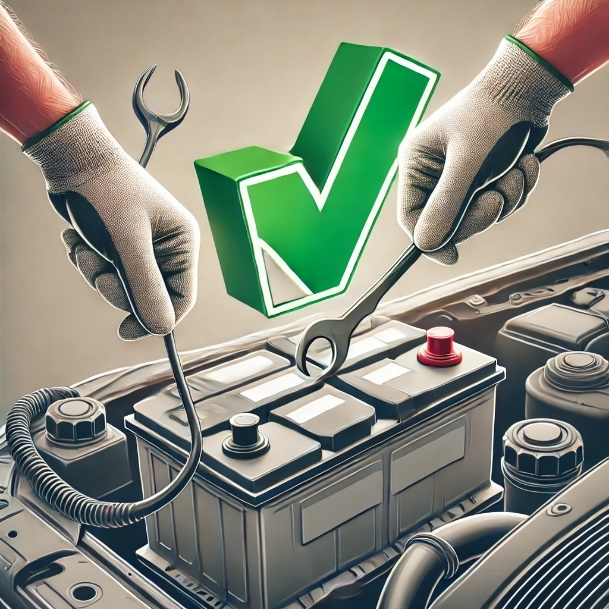
\includegraphics[width=\linewidth]{digifiz_manual/image001.jpg}
        \caption{Címke, amely az akkumulátor lecsatlakoztatására figyelmeztet a beszereléskor.}
    \end{subfigure}\hfill
    \begin{subfigure}{0.46\textwidth}
        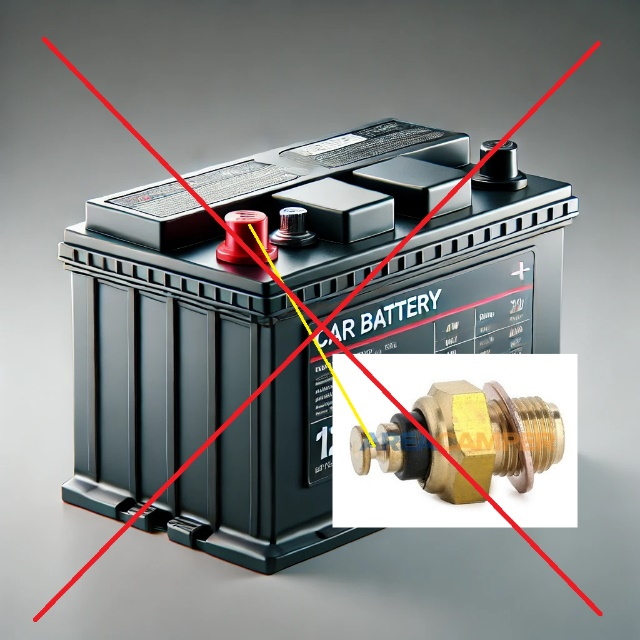
\includegraphics[width=\linewidth]{digifiz_manual/image002.jpg}
        \caption{Figyelmeztetés a szenzorköteghez mellékelve a külső feszültség alkalmazása ellen.}
    \end{subfigure}
    \caption{Biztonsági piktogramok, amelyek a kábelköteggel együtt érkeznek.}
\end{figure}
